\documentclass[8pt]{beamer} 
%\usepackage{pgf}
\usepackage{animate}
\usepackage{graphicx}
\usepackage{subfigure}

\usepackage[utf8]{inputenc}
\usepackage[T1]{fontenc}
\usepackage{lmodern}

\usepackage{amssymb,amsmath,amscd,amsfonts,amsthm,bbm,bm}
\usepackage{wasysym}
%\usepackage{graphicx}
%\usepackage{animate}
%\usepackage{psfrag}
%\usepackage{paralist}
\usepackage{color}
%\usepackage{float}
%\usepackage{relsize}
%\usepackage{euscript}
%\usepackage{setspace}
%\usepackage{flushend}
%%\usepackage[usenames,dvipsnames]{xcolor}
\usepackage{tikz}

\usepackage{pgfplots}
\usetikzlibrary{arrows,shapes,decorations,backgrounds}
\usepackage{tkz-berge}
\DeclareMathOperator*{\argmin}{argmin}
\DeclareMathOperator*{\argmax}{argmax}
\newcommand{\SNR}{\mathsf{SNR}}
\newcommand{\Q}{\mathbb{Q}}
% *** TPT STYLE ***

\setbeamerfont{subsection in toc}{size=\large}

\definecolor{colorframetitle}{RGB}{191,18,56} % Title of frames
\definecolor{redbox}{RGB}{191,18,56} % 
\definecolor{blackbox}{RGB}{0,0,0} % 
\definecolor{brownbox}{RGB}{128,99,90} % 

\usepackage[absolute,overlay]{textpos}
\usepackage{listings}
\usepackage{hyperref}

\setlength{\TPHorizModule}{1mm}
\setlength{\TPVertModule}{1mm}

\usepackage{tikz}
\usetikzlibrary{decorations.pathreplacing,calc}
\usetikzlibrary{arrows,shapes,snakes,automata,backgrounds,petri}
\usepackage{scalefnt}



\newcommand{\tikzmark}[1]{\tikz[overlay,remember picture] \node (#1) {};}

\tikzstyle{mybox} = [draw=redbox, fill=redbox!20, very thick,
    rectangle, rounded corners, inner sep=10pt, inner ysep=20pt]
\tikzstyle{fancytitle} =[fill=redbox, text=white, rectangle]


\newcommand{\MyLogo}{
%\begin{textblock}{14}(117.2,0.7)
\begin{textblock}{14}(108.8,86)

\includegraphics[width=0.8cm]{figures/tpt}

\includegraphics[width=1.1cm]{figures/cisco.png}
 \end{textblock}
}


%\begin{textblock}{14}(117.2,0.7)








\usepackage{beamerthemesplit}

\setbeamercolor{itemize item}{fg=redbox}
\setbeamercolor{structure}{fg=redbox, bg=red}
\setbeamercolor{block title}{bg=brownbox,fg=white}
\setbeamercolor{block title alerted}{bg=redbox,fg=white}
\setbeamercolor{block body alerted}{bg=brownbox!0,fg=black}
\setbeamercolor{block title example}{bg=black, fg=white}
\setbeamercolor{palette primary}{fg=black,bg=white} % changed this
\setbeamercolor{palette secondary}{use=structure,fg=structure.fg!100!white} % changed this
\setbeamercolor{palette tertiary}{use=structure,fg=structure.fg!100!white} % changed this
\setbeamercolor*{palette quaternary}{fg=black,bg=white} % outline on top left
\setbeamercolor{background canvas}{bg=white, fg=black} 
\setbeamercolor{frametitle}{fg=colorframetitle}


% First  frame
\newcommand{\RectanglesOfMainSlide}{%
\raisebox{0mm}[0pt][0pt]{%
\begin{pgfpicture}{0mm}{0mm}{0mm}{0mm}
\pgfsetlinewidth{5mm}
\color{redbox}
\pgfline{\pgfpoint{-4mm}{-12mm}}{\pgfpoint{24mm}{-12mm}}
\color{blackbox}
\pgfline{\pgfpoint{24mm}{-12mm}}{\pgfpoint{52mm}{-12mm}}
\color{brownbox}
\pgfline{\pgfpoint{52mm}{-12mm}}{\pgfpoint{80mm}{-12mm}}
\end{pgfpicture}}}

\newcommand{\makeFirstFrame}{
\setbeamertemplate{footline}{} 
\frame[plain]{
\begin{columns}[c]
\column{3cm}
\vspace{-2cm}\\

\includegraphics[width=1.5cm]{figures/tpt}

\includegraphics[width=2.2cm]{figures/cisco.png}\\
\column{7cm}
\vspace{1cm}\\
\LARGE{\textbf{\theTitle}}\\
\vspace{0.5cm}
\normalsize{\theAuthors}\\
\vspace{0.5cm}
\normalsize{\theResponsible}\\
\vspace{0.5cm}

\normalsize{\theConferenceAndPlace}\\
\vspace{-1cm}
\RectanglesOfMainSlide
\end{columns}
}
\activateFootline
}


% Frames decoration

\newcommand{\RectanglesBeforeTitle}{%
\raisebox{0mm}[0pt][0pt]{%
\begin{pgfpicture}{0mm}{0mm}{0mm}{0mm}
\pgfsetlinewidth{5mm}
\color{redbox}
\pgfline{\pgfpoint{-2mm}{2.2mm}}{\pgfpoint{4mm}{2.2mm}}
\color{blackbox}
\pgfline{\pgfpoint{4mm}{2.2mm}}{\pgfpoint{10mm}{2.2mm}}
\color{brownbox}
\pgfline{\pgfpoint{10mm}{2.2mm}}{\pgfpoint{16mm}{2.2mm}}
\end{pgfpicture}}}

\setbeamertemplate{frametitle}{
\begin{columns}[t]
\column{16mm}
\RectanglesBeforeTitle 
\column{10.7cm}
\strut\textbf{\insertframetitle}\strut
\end{columns}
}

% Foot line

\newcommand{\Ffootline}{
\MyLogo
\begin{tikzpicture}
 \fill [color=white, fill=redbox] (-1, -0.05) rectangle (1, 0.30);
\node[white, right] (note1) at (-1, 0.10) {\insertframenumber/\inserttotalframenumber};
\node[white, left] (note1bis) at (0.98, 0.10) {\theDate};
 \fill [color=white, fill=blackbox] (1.05, -0.05) rectangle (4.5, 0.30);
\node[white, align=center] (note2) at (2.27, 0.12) {Institut Mines-Telecom};
 \fill [color=red, fill=brownbox] (3.55, -0.05) rectangle (9.75, 0.30);
\node[white, align = center] (note3) at (6.65, 0.10) {\thefootnotedef};

%\node[white] (note3) at (7.5, 0.10) {\theTitle};
\end{tikzpicture}
}

\newcommand{\activateFootline}{
\setbeamertemplate{footline}{
\usebeamerfont{structure}
\Ffootline
}
}


% *** END OF TPT STYLE ***


%remove navigation symbols
\setbeamertemplate{navigation symbols}{}

% To show the outline at the beginning of each section
\AtBeginSection[]{
   \begin{frame}
   \frametitle{Plan}
   %\begin{center}{\LARGE Outline }\end{center}
   \tableofcontents[currentsection,hideothersubsections]
   \end{frame} 
}

\newcommand{\mytilde}{\raise.17ex\hbox{$\scriptstyle\mathtt{\sim}$}}

\newcommand{\tikzgrid}{
\begin{pgfonlayer}{background}
\draw[gray!50]
(current bounding box.south west)
grid[step=.2] (current bounding box.north east);
\draw[red!50]
(current bounding box.south west)
grid (current bounding box.north east);
\end{pgfonlayer}
}

\newcommand*{\ExtractCoordinate}[3]{\path (#1); \pgfgetlastxy{#2}{#3};}%

\newdimen\tlx
\newdimen\tlx
\newdimen\brx
\newdimen\bry

%% To FILL to customize presentation with the TPT style

\newcommand{\theTitle}{Routing Algorithms in NDN Networks}
\newcommand{\thefootnotedef}{Routing Algorithms in NDN networks}
\newcommand{\theAuthors}{shahab SHARIAT BAGHERI}
\newcommand{\theResponsible}{Luca MUSCARIELLO\\Beatrice PESQUET \\ Pablo PIANTANIDA}
\newcommand{\theConferenceAndPlace}{Internship Defense \\
Salle F801, TELECOM ParisTech}
\newcommand{\theDate}{9/26/2016}

%%%%%%

\DeclareMathOperator{\tr}{Tr}
\DeclareMathOperator{\support}{supp}
\DeclareMathOperator{\rank}{rank}
\DeclareMathOperator{\diag}{diag}
\newcommand{\bs}{\boldsymbol}

% Convergences 
\newcommand{\toaslong}{\xrightarrow[T\to\infty]{\text{p.s.}}}
\newcommand{\toasshort}{\xrightarrow{\text{p.s.}}}
\newcommand{\toprobalong}{\xrightarrow[T\to\infty]{{\cal P}}}
\newcommand{\toprobashort}{\xrightarrow{{\mathcal P}}}
\newcommand{\tolawlong}{\xrightarrow[T\to\infty]{{\cal L}}}
\newcommand{\tolawshort}{\xrightarrow{{\mathcal L}}}
\newcommand{\tolong}{\xrightarrow[T\to\infty]{}}
\newcommand{\norme}[1]{\left\Vert #1\right\Vert}

% Notations bb 
\newcommand{\N}{\mathbb N}
\newcommand{\R}{\mathbb R}
\newcommand{\Z}{\mathbb Z}
\newcommand{\C}{\mathbb{C}}
\newcommand{\E}{\mathbb{E}}
\newcommand{\1}{\mathbbm 1}
\newcommand{\PP}{\mathbb{P}}
 
\newcommand{\bl}{\{} 
\newcommand{\br}{\}} 

\def\bx{{\bf x}}\def\bx{{\bf x}}

\def\bA{{\bf A}}
\def\bY{{\bf Y}}
\def\bV{{\bf V}}
\def\bQ{{\bf Q}}
\def\ba{{\bf a}}
\def\bc{{\bf c}}
\def\bd{{\bf d}}
\def\bm{{\bf m}}
\def\bg{{\bf g}}
\def\bp{{\bf p}}
\def\bv{{\bf v}}
\def\bx{{\bf x}}
\def\by{{\bf y}}
\def\brho{{\boldsymbol \rho}}
\def\bDelta{{\boldsymbol \Delta}}
\def\bdelta{{\boldsymbol \delta}}

\def\bOmega{{\bf \Omega}}
\def\bbT{{\bf \mathbb{T}}}

\newtheorem{assumption}{Assumption}

\newcommand{\semitransp}[2][35]{\color{fg!#1}#2}

\begin{document}
 

 
\makeFirstFrame

\frame{
  \frametitle{Plan}
  \tableofcontents
}

\setbeamertemplate{blocks}[rounded][shadow=true]
\section{Internship Environment}

%%%%%%%%%%%%%%%%%%%%%%%%%%%%%%%
\subsection{CISCO \& PIRL}

\begin{frame}{CISCO \& PIRL}

Cisco Systems France.

\begin{center}
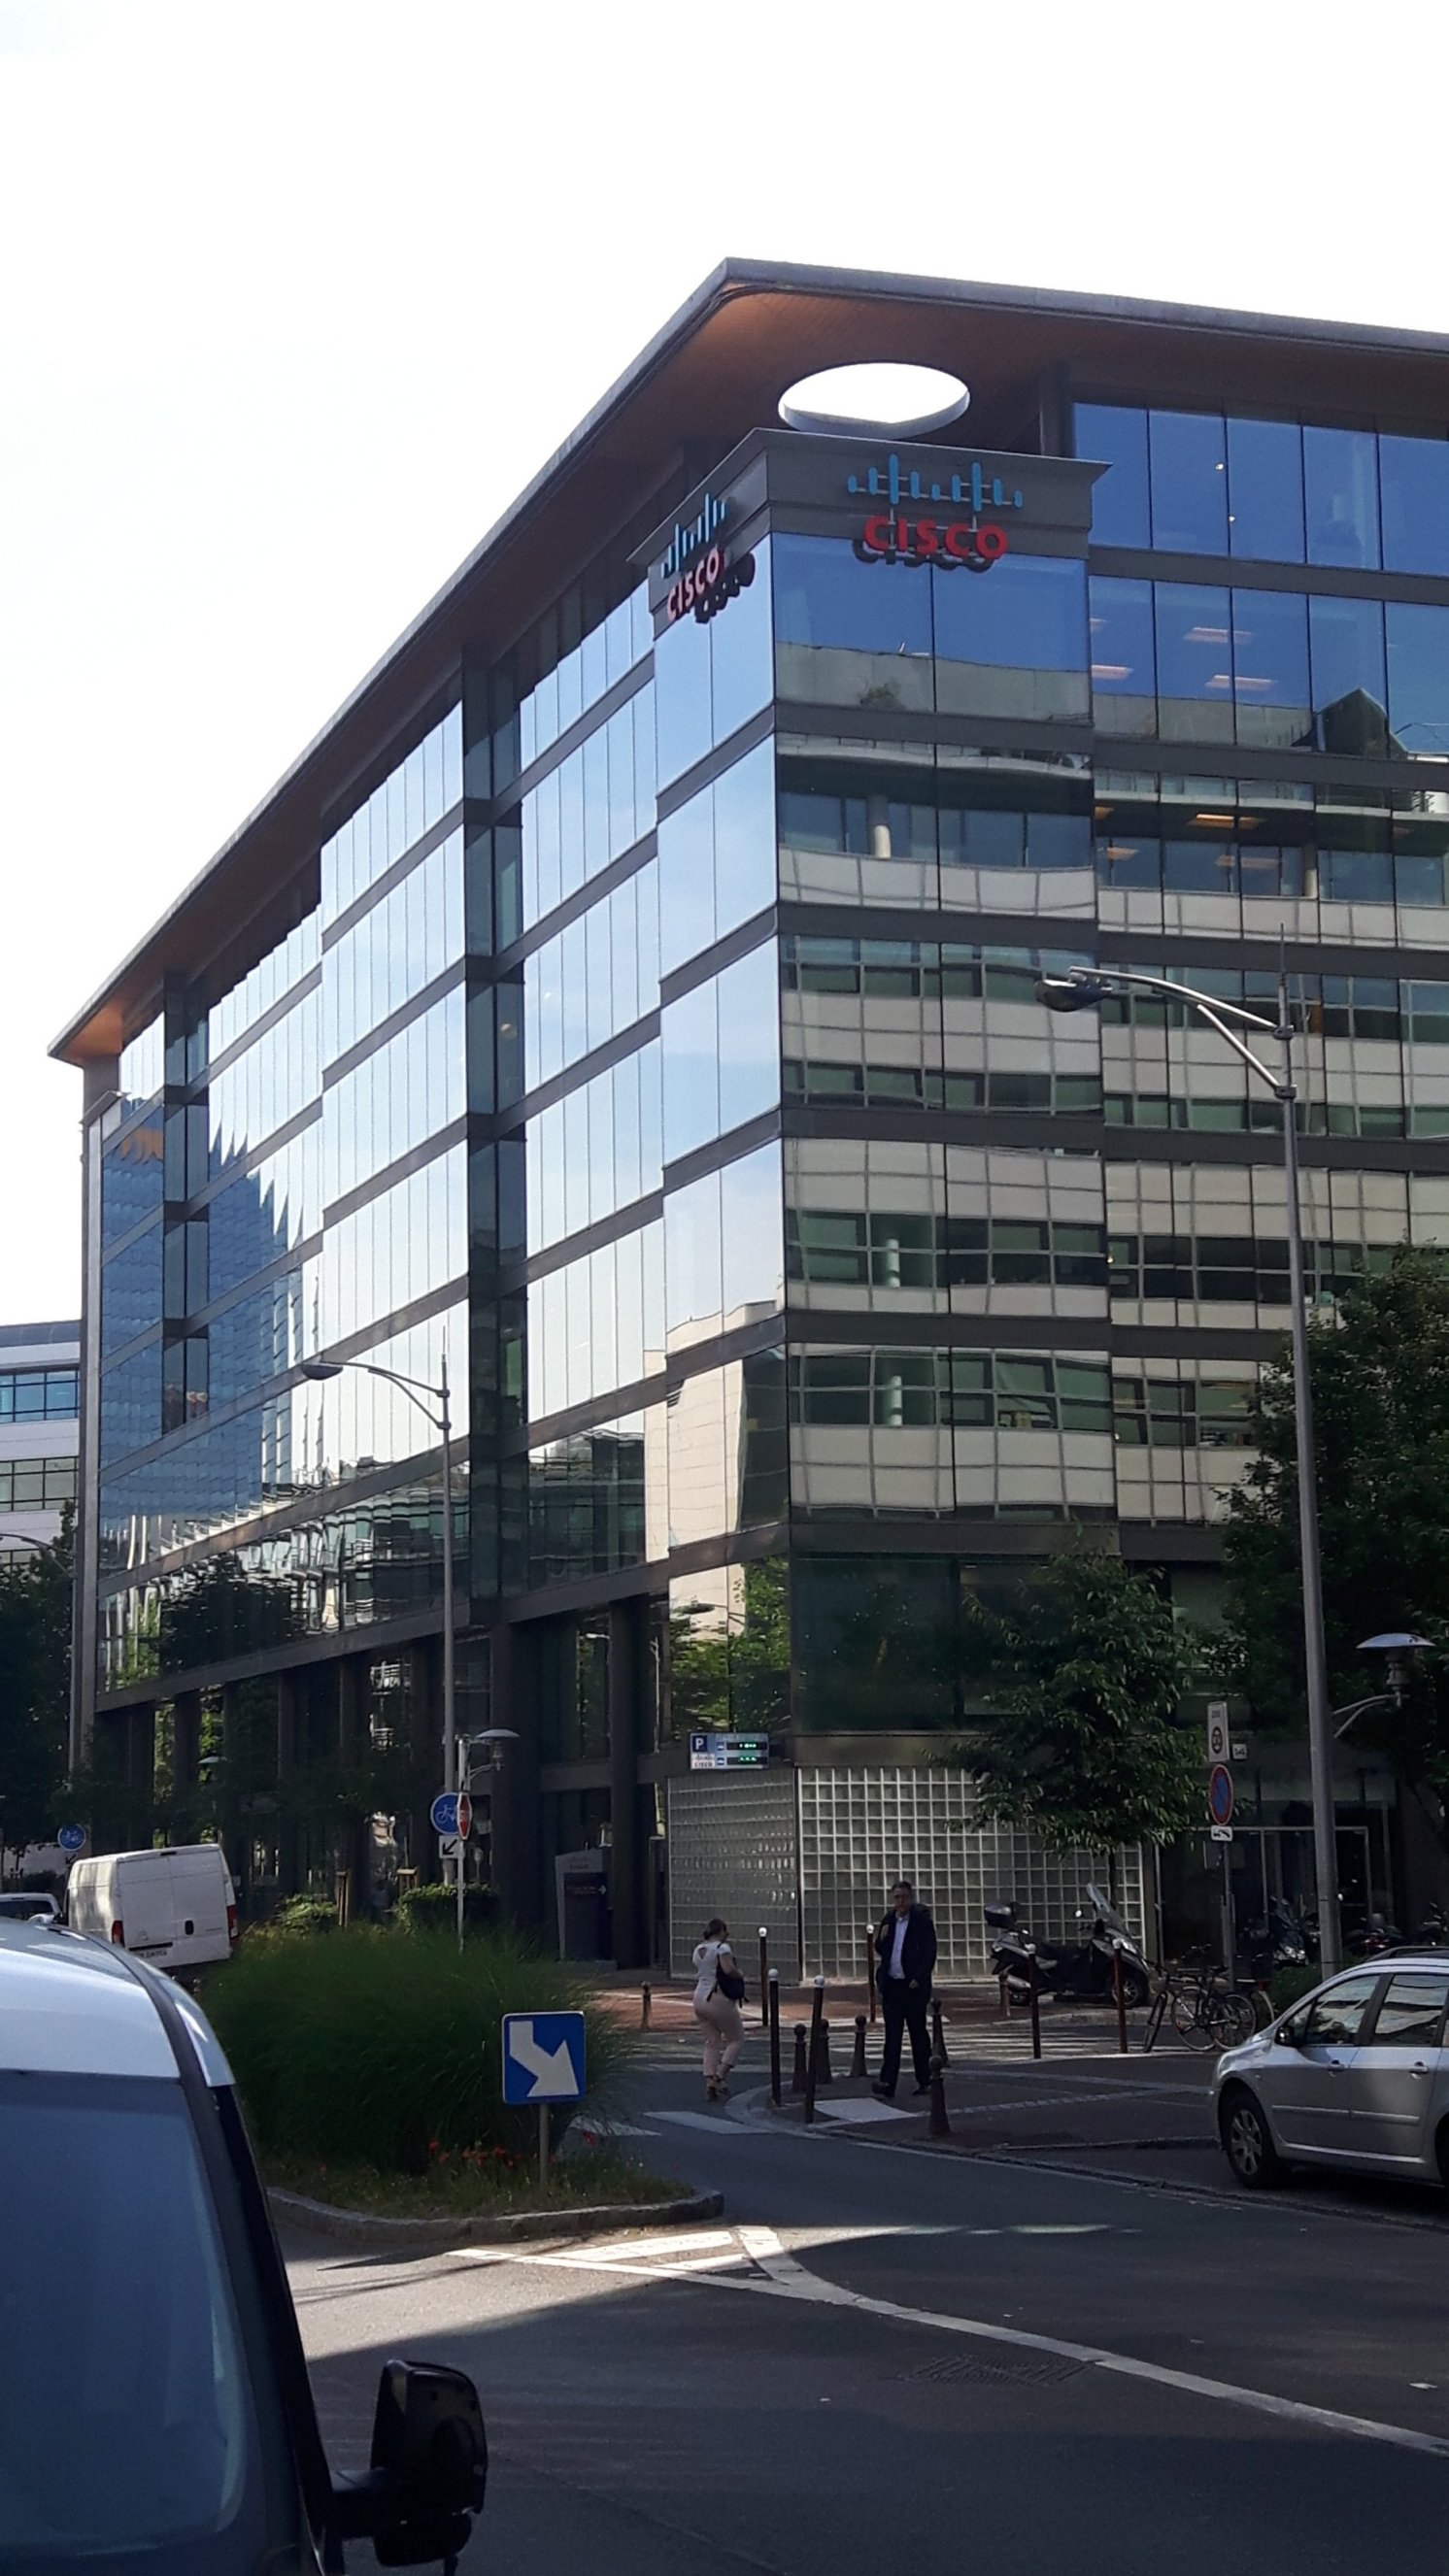
\includegraphics[scale=0.07]{figures/cisco.jpg}
\end{center}


\end{frame}

\begin{frame}{PIRL}

\textbf{P}aris \textbf{I}nnovation and and \textbf{R}esearch \textbf{L}aboratory.

\begin{center}
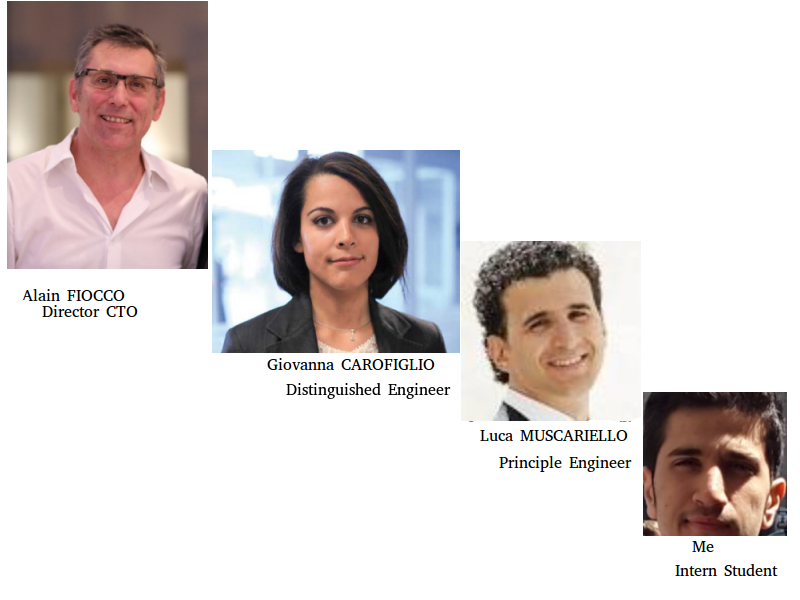
\includegraphics[scale=0.22]{figures/photos.png}
\end{center}



\end{frame}




%%%%%%%%%%%%%%%%%%%%%%%%%%%%%%%

\subsection{Goals and objectives}
\begin{frame}{Goals and objectives}

\only<1>{
Net Revenu for Video Delivery Applications

\begin{center}
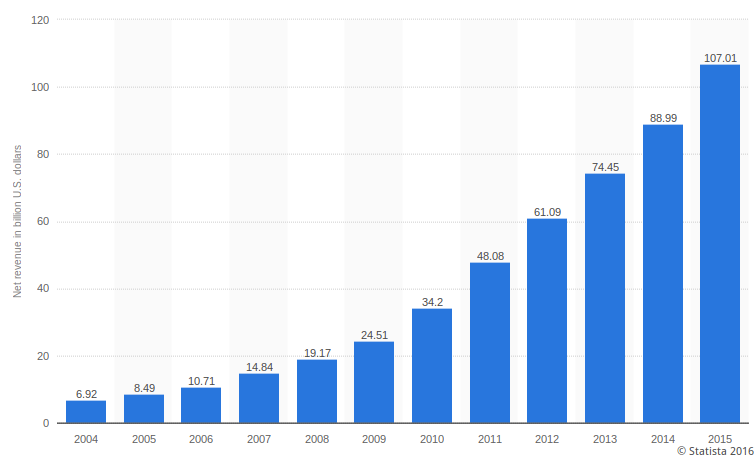
\includegraphics[scale=0.28]{figures/amazon.png}
\end{center}
}

\only<2>{
In 2016, More than 96 \% of internet traffic is content.

Video $\longrightarrow$ 60\%

File sharing $\longrightarrow$ 20\%

Web $\longrightarrow$ 20\%

\begin{center}
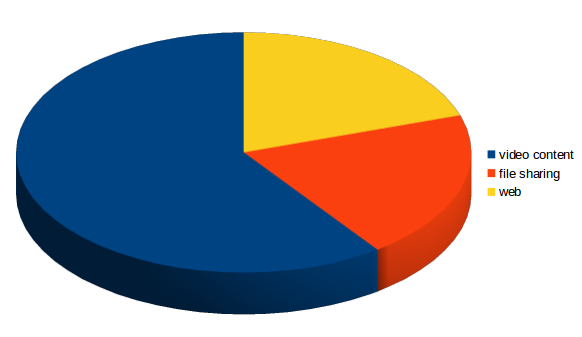
\includegraphics[scale=0.28]{figures/stat.png}
\end{center}

}

\only<3>{
Mobile vs PC Internet Traffic user $\longrightarrow$ 5G mobile networks


\begin{center}
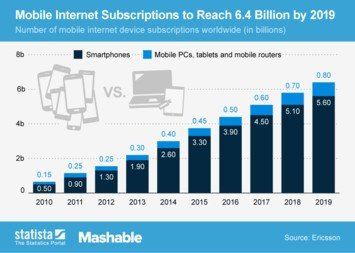
\includegraphics[scale=0.48]{figures/mobile.jpg}
\end{center}

}




\end{frame}

%%%%%%%%%%%%%%%%%%%%%%

%\subsection{Interference Alignment Techniques}
%\begin{frame}
%\frametitle{Interference Alignment Techniques}
%\vspace{-0.65cm}
%\uncover<1->{
%  \begin{block}{Which techniques to be used for IA ?}
%  \centering
%  \begin{itemize}
%  \item Linear Lattice-based Interference Alignment. 
%  \item The Compute-and-Forward (CoF) method described by [Nazer and Gastpar 2008].
%  \end{itemize}
%\end{block}}
%\vspace{-0.31cm}
%\uncover<2->{\begin{block}{Recent Research Studies ...}
%   \begin{itemize}
%   \item A coding scheme presented by [Khaleghi and Belfiore 2014] to improve the fading behavior of achievable sum rates defined in [Ordentlich \textit{et al.} 2012].
%   \item Lattice codes over Eisenstein integers presented for CoF [Tunali \textit{et al.} 2012] to achieve higher rates.
%   \end{itemize}}
%   \vspace{-0.15cm}
%   \uncover<3->{
%  For the \underline{complex-valued interference channels} need to realize more research.}
%  \vspace{0.1cm}
%  \uncover<4->{\\$\rightarrow$ In this research we focus on \textcolor{red}{\textit{the complex-valued interference channels}} and employing $\Z[i]$-lattice codes.
%   \end{block}}
%   \vspace{-0.31cm}
% \uncover<5->{
%   \begin{block}{In Compute-and-Forward scheme [Receiver's Point of View]}
%    \centering
%    \begin{enumerate}
%     \item Receiving linear combination of the transmitted codewords.
%     \item Deciding which equation(s) to be decoded.}
%     \uncover<6->{
%     \item Applying the corresponding Minimum Mean Square Error estimation (MMSE).
%     \item Decoding the equation(s) in $\Lambda_{\textrm{lattice}}$.
%    \end{enumerate}
%   \end{block}}
%\end{frame}

%%%%%%%%%%%%%%%%%%%%%%%
\section{Ideas and Strategies}

\subsection{ICN Brief Introduction}

\begin{frame}{Named Data networking (NDN)}

\begin{itemize}
\item V.Jacobson et al proposition, \textit{Networking Named Content} 2009.

\item \textbf{I}nformation \textbf{C}entric \textbf{N}etworking $\Rightarrow$ \textit{\textbf{Name}} base Philosophy vs IP \textit{\textbf{Calling}} Networking.

\item A Good fit network desiging for Video Delivery Applications in \textbf{5G}.

\end{itemize}
\only<1>{
\begin{center}
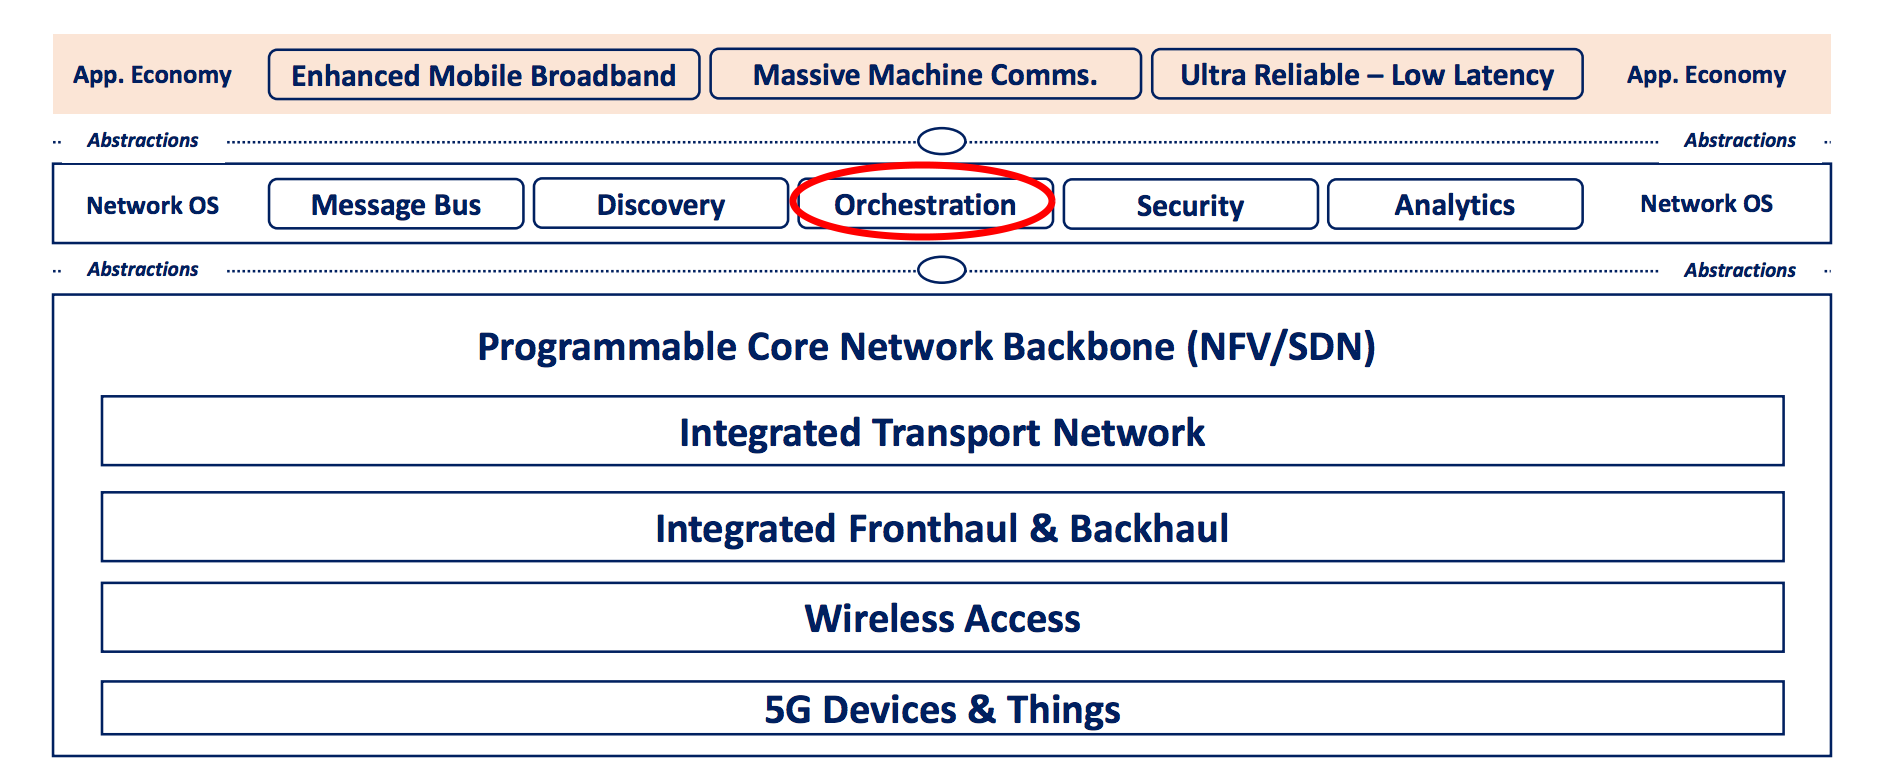
\includegraphics[scale=0.28]{figures/architecture.png}
\end{center}
}

\only<2>{
\begin{center}
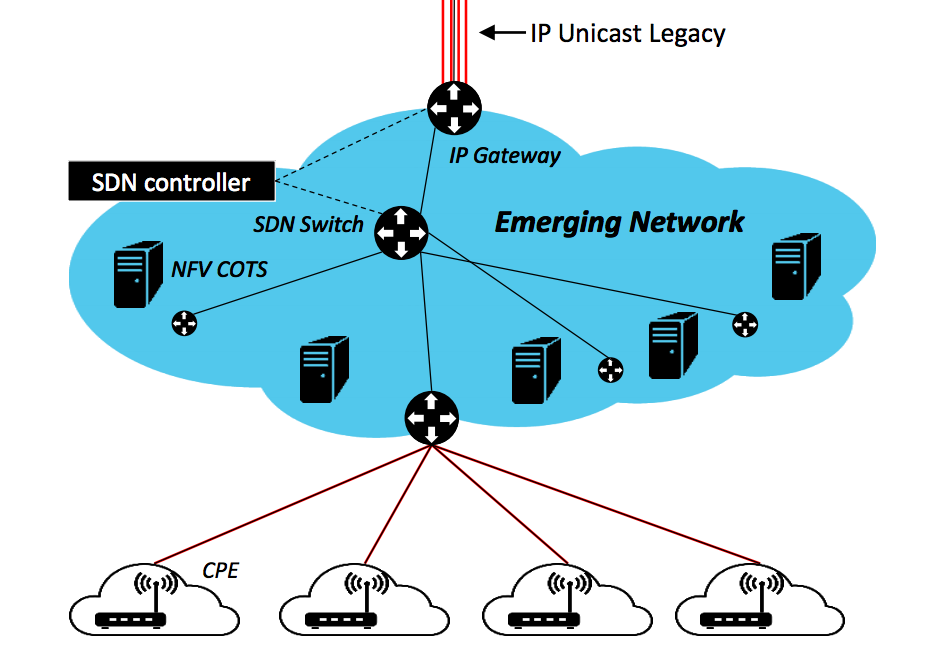
\includegraphics[scale=0.28]{figures/sdn.png}
\end{center}
}



\end{frame}





\subsection{Virtualization and Linux Containers}

\subsubsection{Choix du Filtre Gaussien}

\begin{frame}{Choix du Filtre Gaussien}
\uncover<1->{
- GFSK modulation $\rightarrow$ $BT$(Paramètre de filtre Gaussien) $=$} \only<1>{1}\only<2>{\textbf{1} $\rightarrow$ Normal-Rate}\only<1>{$,0.5, 0.3$}
\only<1>{
\begin{itemize}
\item Bit Error Rate
\item Intérference entre canaux adjacents
\end{itemize}
\begin{figure}
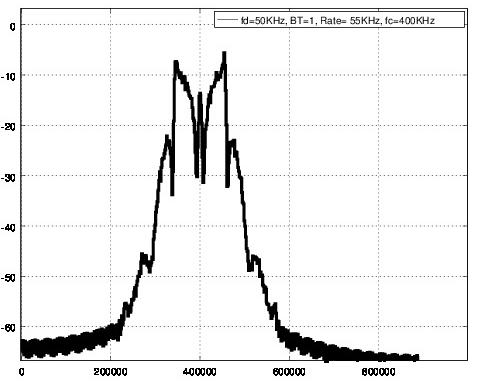
\includegraphics[scale=0.22]{figures/fig1.jpg}
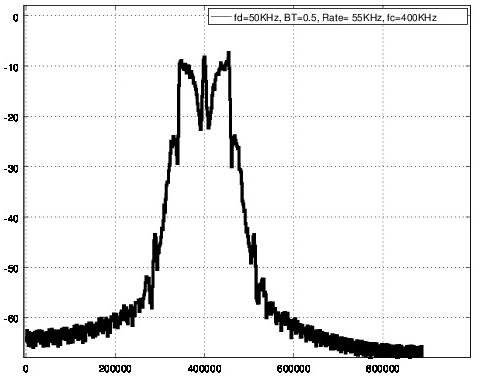
\includegraphics[scale=0.22]{figures/fig2.jpg} \\
\centering
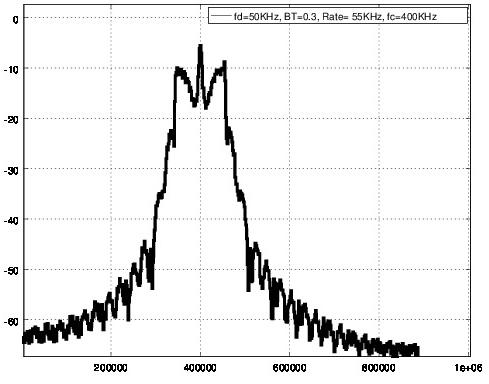
\includegraphics[scale=0.22]{figures/fig3.jpg} 
\end{figure}}
\only<2>{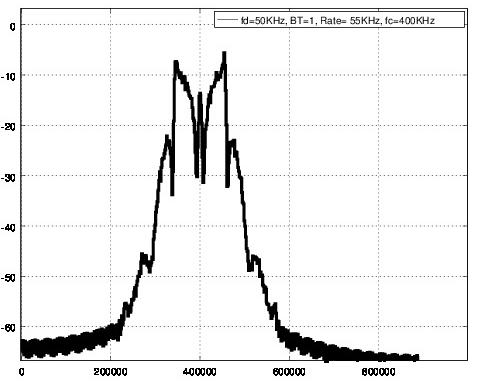
\includegraphics[scale=0.5]{figures/fig1.jpg}}
%  \vspace{-0.6cm}
%  \uncover<1->{
%  \begin{block}{Channel Model}
%  \centering
%  The channel model is : the \textit{K}-User Gaussian Symmetric Complex-Valued Interference Channel (GS-CIC).
%  \begin{itemize}
%   \item By using a simple lattice IA [Ordentlich \textit{et al.} 2012], the \textit{K}-User case will be approximately equivalent to a 2-User case.
%   \end{itemize}
%   \begin{equation}
%    \label{Channel_Mod}
%    \mathbf{y}=H\mathbf{x}+\mathbf{z},\hspace{0.1cm}
%    with\hspace{0.1cm}H=\left[\begin{array}{cc} 1 & g\\ g & 1 \end{array}\right]
%    \end{equation}
%    
%    \begin{minipage}{0.4\textwidth}
%    \begin{flushleft}{
%    $\mathbf{y}:$ The output-vector of size 2.\\
%    $\mathbf{x}:$ The input-vector of size 2.\\
%    $\mathbf{z}:$ The noise-vector of size 2. (With $\mathcal{CN}\left(0,{\sigma}^2\right)$)\\ 
%    $g:$ Complex-valued channel interferer coefficient. \\(With $g=\rho e^{i\phi}\in\C$)}
%    \end{flushleft}
%    \end{minipage}
%    \begin{minipage}{0.5\textwidth}
%    \vspace{-0.2cm}  
%    
%    \begin{figure}[h]
%    \centering
%    \begin{tikzpicture}[scale=0.7]
%
%      \draw (0,0) rectangle (0.7,-0.7);
%      \node at (-0.75,-0.35) {$w_1$};
%      \draw [->] (-0.52,-0.35)--(0,-0.35);  
%      \node at (0.35,-0.35) {$\mathcal{E}_1$};
%      \draw [->] (0.7,-0.35)--(2.25,-0.35); 
%      \node at (0.4,-0.95) {$\mathrm{TX}_1$}; 
%      \node at (0.9,-0.15) {${x}_1$};
%      \draw (2.4,-0.35) circle [radius=0.15];
%      \draw  (2.3,-0.35)--(2.5,-0.35);
%      \draw (2.4,-0.25)--(2.4,-0.45);
%      \node at (1.8,-0.15) {$1$};
%      \node at (2.45,0.25) {${z}_1$};  
%      \draw [->] (2.4,0.18)--(2.4,-0.2); 
%      \draw [->] (2.55,-0.35)--(3.25,-0.35); 
%      \node at (3,-0.15) {${y}_1$};
%      \draw (3.25,0) rectangle (3.95,-0.7);
%      \node at (3.6,-0.35) {$\mathcal{D}_1$};
%      \node at (3.65,-0.95) {$\mathrm{RX}_1$}; 
%      \draw [->] (3.95,-0.35)--(4.47,-0.35); 
%      \node at (4.7,-0.3) {$\hat{w}_1$};
%                              
%      \draw (0,-2) rectangle (0.7,-2.7);
%      \node at (-0.75,-2.35) {${w}_2$};
%      \draw [->] (-0.52,-2.35)--(0,-2.35);  
%      \node at (0.35,-2.35) {$\mathcal{E}_2$};
%      \draw [->] (0.7,-2.35)--(2.25,-2.35); 
%      \node at (0.4,-2.95) {$\mathrm{TX}_2$}; 
%      \node at (0.9,-2.15) {${x}_2$};
%      \draw (2.4,-2.35) circle [radius=0.15];
%      \draw  (2.3,-2.35)--(2.5,-2.35);
%      \draw (2.4,-2.25)--(2.4,-2.45);
%      \node at (1.8,-2.15) {$1$};
%      \node at (2.45,-1.75) {${z}_2$};  
%      \draw [->] (2.4,-1.82)--(2.4,-2.2); 
%      \draw [->] (2.55,-2.35)--(3.25,-2.35); 
%      \node at (3,-2.15) {${y}_2$};
%      \draw (3.25,-2) rectangle (3.95,-2.7);
%      \node at (3.6,-2.35) {$\mathcal{D}_2$};
%      \node at (3.65,-2.95) {$\mathrm{RX}_2$}; 
%      \draw [->] (3.95,-2.35)--(4.47,-2.35); 
%      \node at (4.7,-2.3) {$\hat{w}_2$};           
%   
%      \draw [->] (1,-0.35)--(2.3,-2.25); 
%      \draw [->] (1,-2.35)--(2.3,-0.45); 
%      \node at (1.27,-1) {$g$}; 
%      \node at (1.3,-1.65) {$g$};
%   
% \end{tikzpicture}
% \vspace{-0.4cm}
% \caption{2-User GS-CFC.}\label{GS-CFC}
% \end{figure}
% \end{minipage}
%    
% \end{block}}
% 
% \vspace{-0.3cm}
% 
% \uncover<2->{
% \begin{block}{Lattice Structure}
% \centering
% $\rightarrow$ We consider the \underline{nested $\Z[i]$-lattice codes} [Ordentlich \textit{et al.} 2012].
% \end{block}}
\end{frame}

%%%%%%%%%%%%%%%%%%%%%
\subsubsection{Routing Strategies}
\begin{frame}{Design Mask}
\textbf{Publié la nouvelle Spécification de DASH7 (Version 1.0), En Mai 2015.}
\begin{figure}
\uncover<1->{
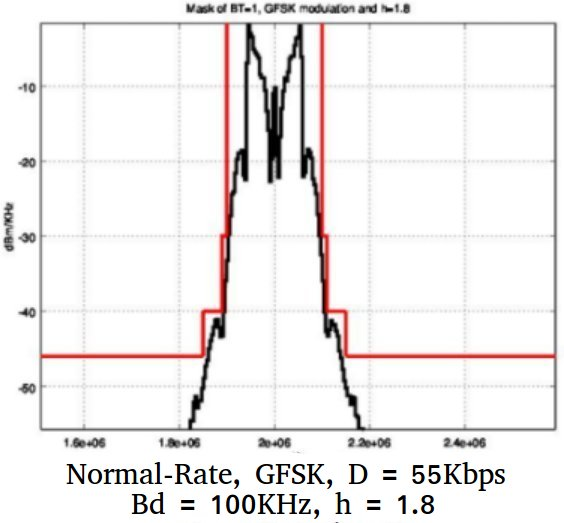
\includegraphics[scale=0.2]{figures/test.jpg}}
\uncover<2->{
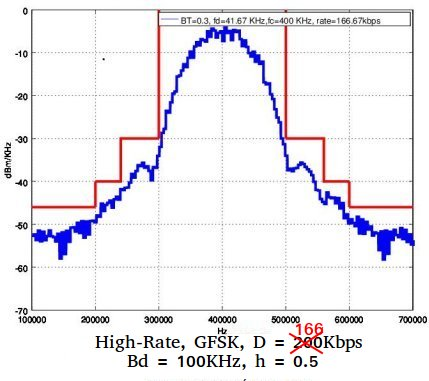
\includegraphics[scale=0.27]{figures/maskhigh.jpg}}
\uncover<3->{
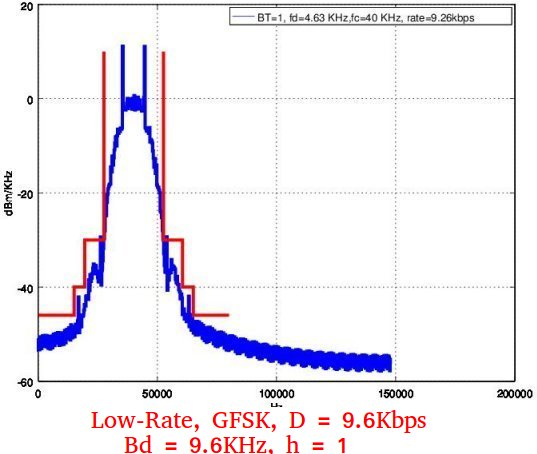
\includegraphics[scale=0.2]{figures/masklow.jpg}$\rightarrow$ Cognitive Radio (SDR)}
\end{figure}

% \vspace{-0.4cm}
% \uncover<1->{
% \begin{block}
% \centering
% \begin{itemize}
% 
%  \item A channel is called symmetric when:\\
%  \begin{center}
%  $H(i,j)=g\hspace{0.1cm}\text{for all}\hspace{0.1cm}{i \not= j}\hspace{0.1cm}\text{and after normalization}\hspace{0.1cm}H(i,j)= 1.$
%  \end{center}
%  
%  \item All the users have the same power constraint, for user $i$ and $n$ channel uses:\\
%  \begin{center}
%  ${\frac{1}{n}} \sum_{j=0}^{n} \vert{\mathbf{x}_{i}}\vert^2 \leq P_\mathrm{i}$
%  \end{center}
%  
%  \vspace{-0.2cm}
%  \item The $\SNR$ is defined as:\\
%  \vspace{-0.2cm}
%  \begin{center}
%  $\SNR=\frac{P}{\sigma^2}$
%  \end{center}
%
%  \item For the 2-User GS-CFC the Interference to Noise Ratio ($\mathsf{INR}$) is defined as:\\
%  \begin{center}
%  $\text{For user i,}\hspace{0.1cm}\mathsf{INR}_{i}=\vert g\vert^2\SNR$
%  \end{center}
%\item The \textit{interference level} is:\\
%\begin{center}
%$\alpha=\frac{\log_{2}(\mathsf{INR_{i}})}{\log_{2}(\SNR)}$
%\end{center}  
%  
%  \end{itemize}
%  \end{block}}
%
% \uncover<2->{
%   \begin{block}
%   \centering
%    \begin{itemize}
%     \item We focus on Strong and Very Strong interference regimes when:\\
%  	 \begin{center}
%     $1<\alpha<2$ and $\alpha\geq2$ 
%  	 \end{center}}
%     \uncover<3->{
%     \item Asymptotic regimes of $\SNR$ are considered (when $\SNR\rightarrow\infty$).}
%     \uncover<4->{
%     \item The Complex-valued channel does not split to two parallel real-valued channels.
%    \end{itemize}
%   \end{block}}
   
\end{frame}

\begin{frame}
\begin{center}
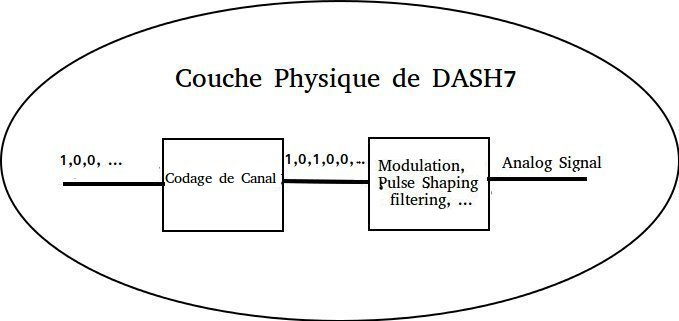
\includegraphics[scale=0.48]{figures/physique.jpg}
\end{center}

\end{frame}
%%%%%%%%%%%%%%%%%%%%%%%%

\subsection{Routing Algorithms}

\subsubsection{Les Codes Proposés}

\begin{frame}{Codages du Canal}
- Les Codes de Contrôle d'erreur 
\begin{itemize}
\item Codage à Détecter les erreurs (CRC, CheckSum, Parité, ...).
\item Codage à Détecter et Corriger les erreurs(LDPC, Convolutif,Turbo, RS, BCH, ...).
\end{itemize}
\begin{block}{Le Concept Principal de Notre Proposition}
Header + Payload + CRC (Convolutif) $\rightarrow$ Header (\textbf{RS}), Payload (\textbf{LDPC}) + CRC 
\begin{itemize}
\item Header: RS $\rightarrow$ La longeur petite
\\-RS(60,28)
\begin{itemize}
\item Encodage: Structure algébrique des polynomials ($g(x)$).
\item Décodage: Error Trapping.
\end{itemize}
\item Payload: LDPC  $\rightarrow$ Pourquoi? 
 
\end{itemize}
\begin{table}
\begin{center}
    \begin{tabular}{| l | l | l |}
    \hline
     Header & Payload & CRC16 \\ \hline
        $ 28 Bit $ & $16-255 Byte$ & $2 Byte$ \\ \hline   
     \end{tabular}
    \end{center}
\end{table}

\end{block}

\end{frame}

%%%%%%%%%%%%%%%
\subsubsection{Les Résultats et les Courbes BLER des Nouveaux Codes}

\begin{frame}{LDPC vs Convolutif dans les expériences et Handbooks ...}
%

\begin{block}{Pourquoi LDPC?}
\begin{itemize}
\item Très proche à la limite de Shannon (0.042dB).
\item Augmentation la taille de Matrice Parité Check $\rightarrow$ Meilleur Performance. 
\item Pour changer le taux on peut juste modifier les lignes.
\item Ils ne sont pas brevetés et très répandu.
\item Application Réseau: 5G, Wi-Fi, IEEE 802.16 (WiMAX), 10GBase-T de Ethernet, DVB-S2, ... .

\end{itemize}
\end{block}

\end{frame}

\begin{frame}{LDPC}

\begin{block}{Choix de LDPC (Méthodes Aléatoires)}

\begin{itemize}
\item En vert: Gallagar,Computer generated, 1963 $\rightarrow$ Dégradation, \textit{girth = 4-cycle} $\rightarrow$  Matrice de \textbf{Génératrice} (Encodage: non complèxe)
 
 
\item En rouge: Mackay-Neal, 1996 \cite{errorcontrolcoding}$\rightarrow$ Eviter les 4-cycles $\rightarrow$ Matrice \textbf{Génératrice} (Encodage: complèxe)
\end{itemize}

\end{block}

\begin{center}
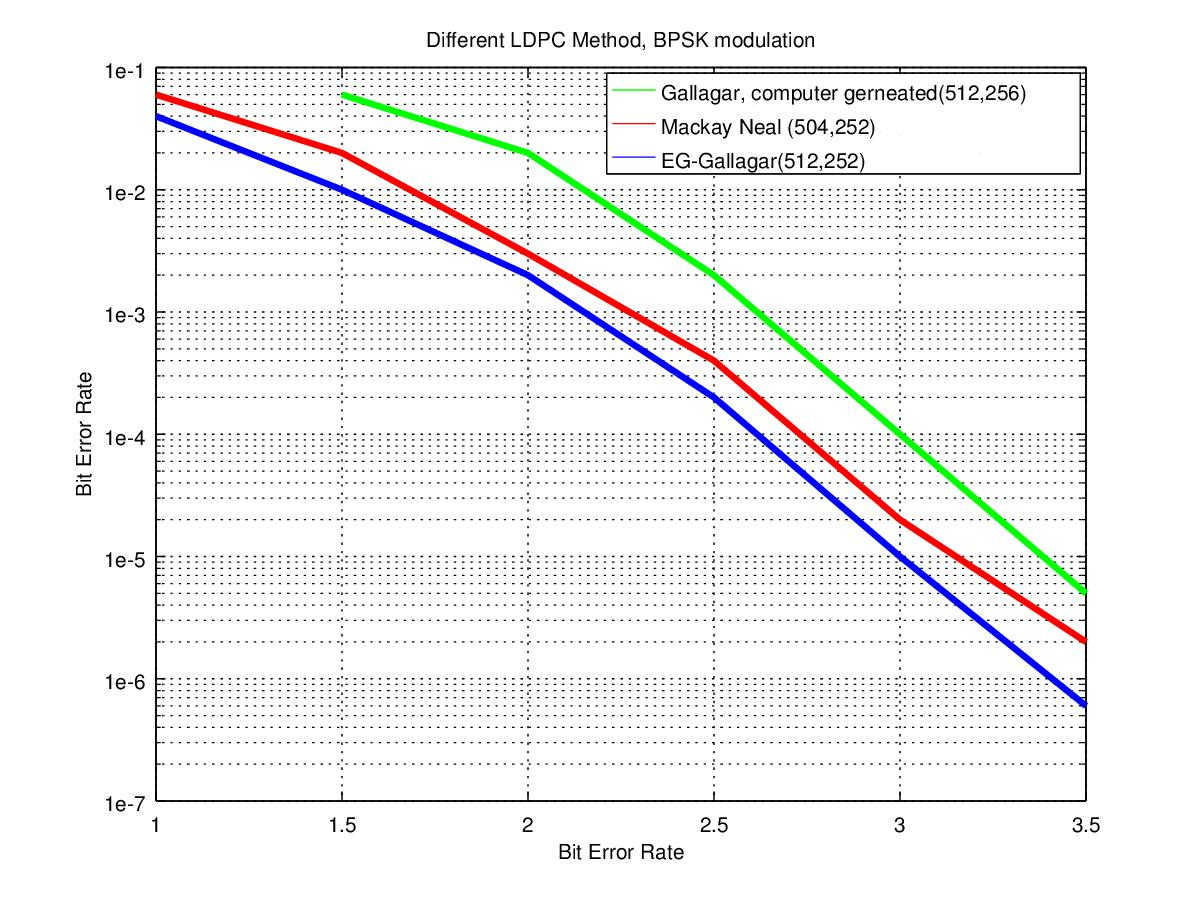
\includegraphics[scale=0.35]{figures/ber_ldpc.jpg}
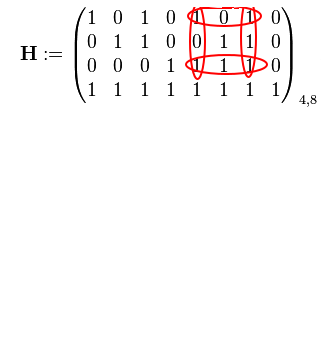
\includegraphics[scale=0.4]{figures/H.png}

\end{center}
\end{frame}

\begin{frame}{LDPC (1/2) vs Convolutif (1/2)}


\only<1>{
\begin{block}{LDPC Contre Convolutif (Encodage)}



- \textbf{LDPC Mackay-Neal}: Complèxe $\rightarrow$ Algorithm de Richardson-Urbanke $\rightarrow$ Diréctement a travers de \textbf{H} --- $O(n^{2})\rightarrow O(n+g^{2})$. 
 

- \textbf{Convolutif}: Circuit de Shift Register.  
 

\end{block}}





\only<2>{
\begin{block}{LDPC Contre Convolutif (Décodage)}

 \textbf{LDPC}: 
 \begin{itemize}
\item Hard: Algorithme de Bit flipping $\rightarrow$ Graph Tanner (iteration = 10) .
\item Soft: Algorithme de Log-DomainSimple (Version simplifiée de l'algorithm SPA) $\rightarrow$ Probabilité a priori (ML)  (iteration = 10)

\end{itemize}

- \textbf{Convolutif}: Algorithm de Viterbi $\rightarrow$ Graph Trellis
 

\end{block}}

\only<4>{

\begin{block}{LDPC(1/2) vs Convolutif(1/2)}
Modèle de canal: AWGN \& TU5 (Typical-Urban)$\rightarrow$ Jakes algorithm



\end{block}



}




\begin{center}
\only<1>{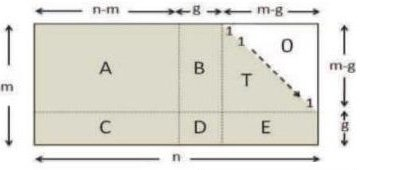
\includegraphics[scale=0.28]{figures/matrix.jpg} 
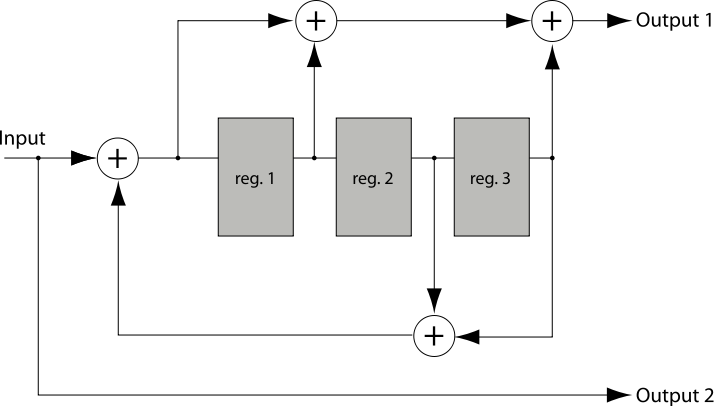
\includegraphics[scale=0.15]{figures/encoder.png}}
\only<2>{
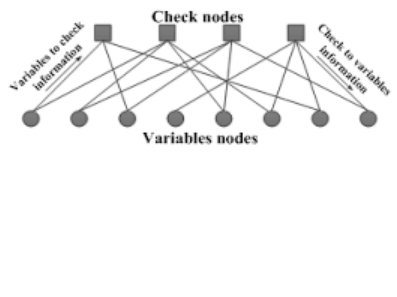
\includegraphics[scale=0.3]{figures/bipartite.jpg}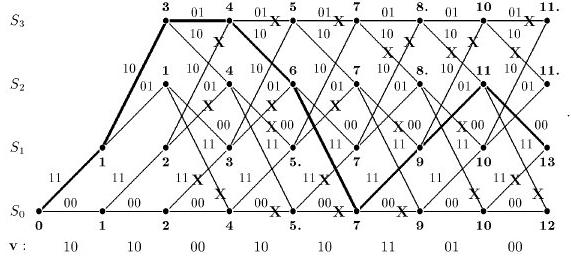
\includegraphics[scale=0.3]{figures/viterbi.jpg}
}
\only<3>{\begin{block}{LDPC vs Convolutif} \begin{center} 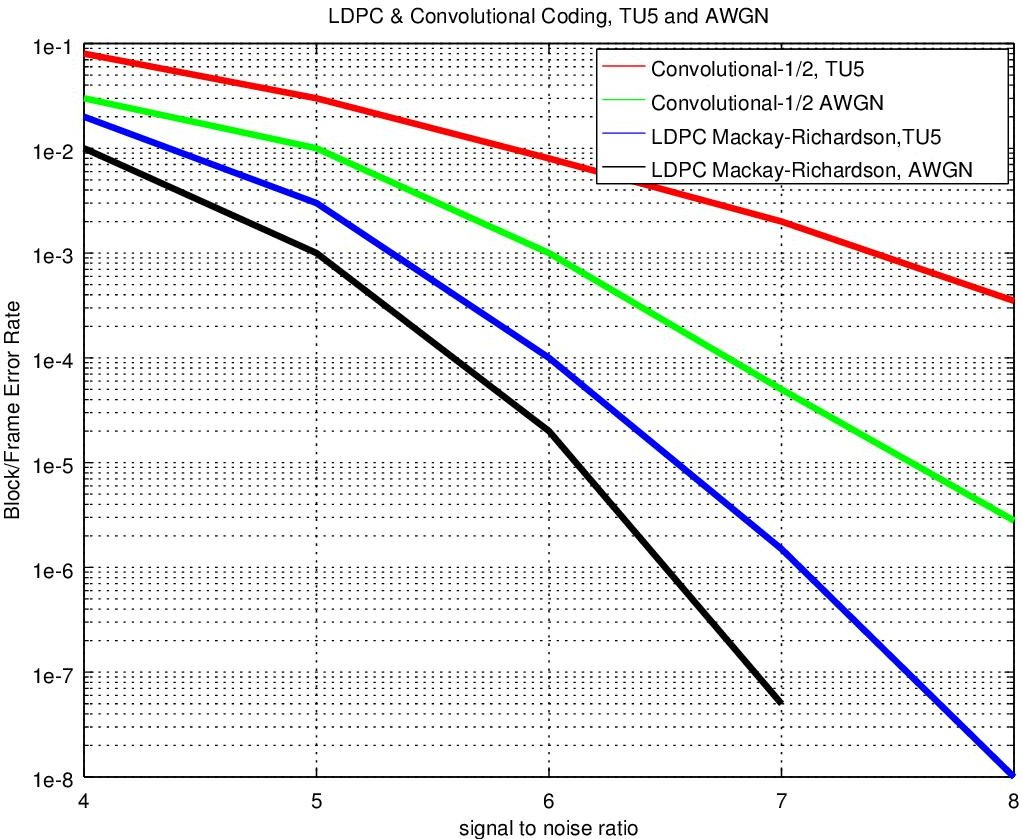
\includegraphics[scale=0.2]{figures/bler_conv.jpg} \end{center} \end{block}}
\only<4>{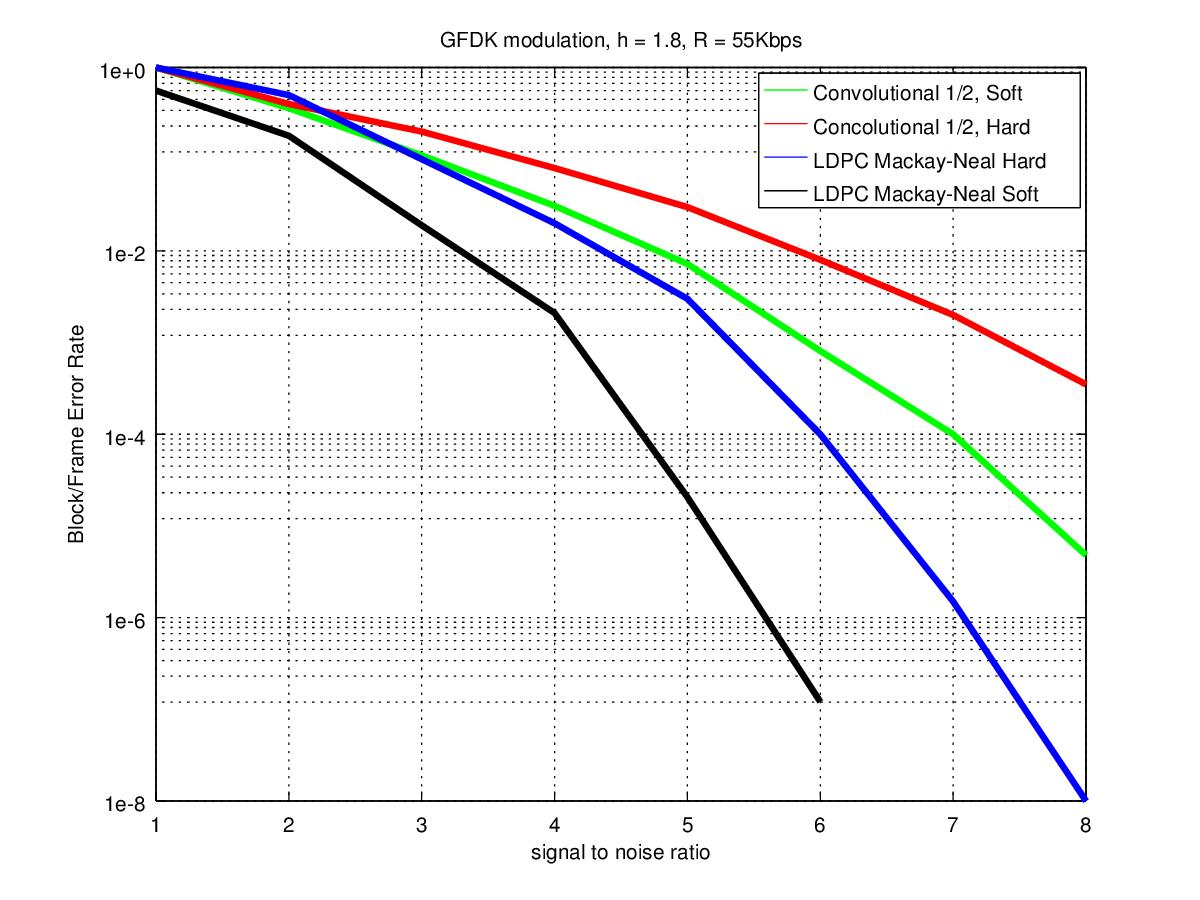
\includegraphics[scale=0.4]{figures/LDPC_Conv_final.jpg}}
\end{center}



\end{frame}







%%%%%%%%%%%%%%%%%%%
%
%\begin{frame}
%\begin{block}{Résultat}
%Codage de Header (RS(60,28)) et Codage de Payload(LDPC(256,128)+CRC)
%\end{block}
%
%\centering
%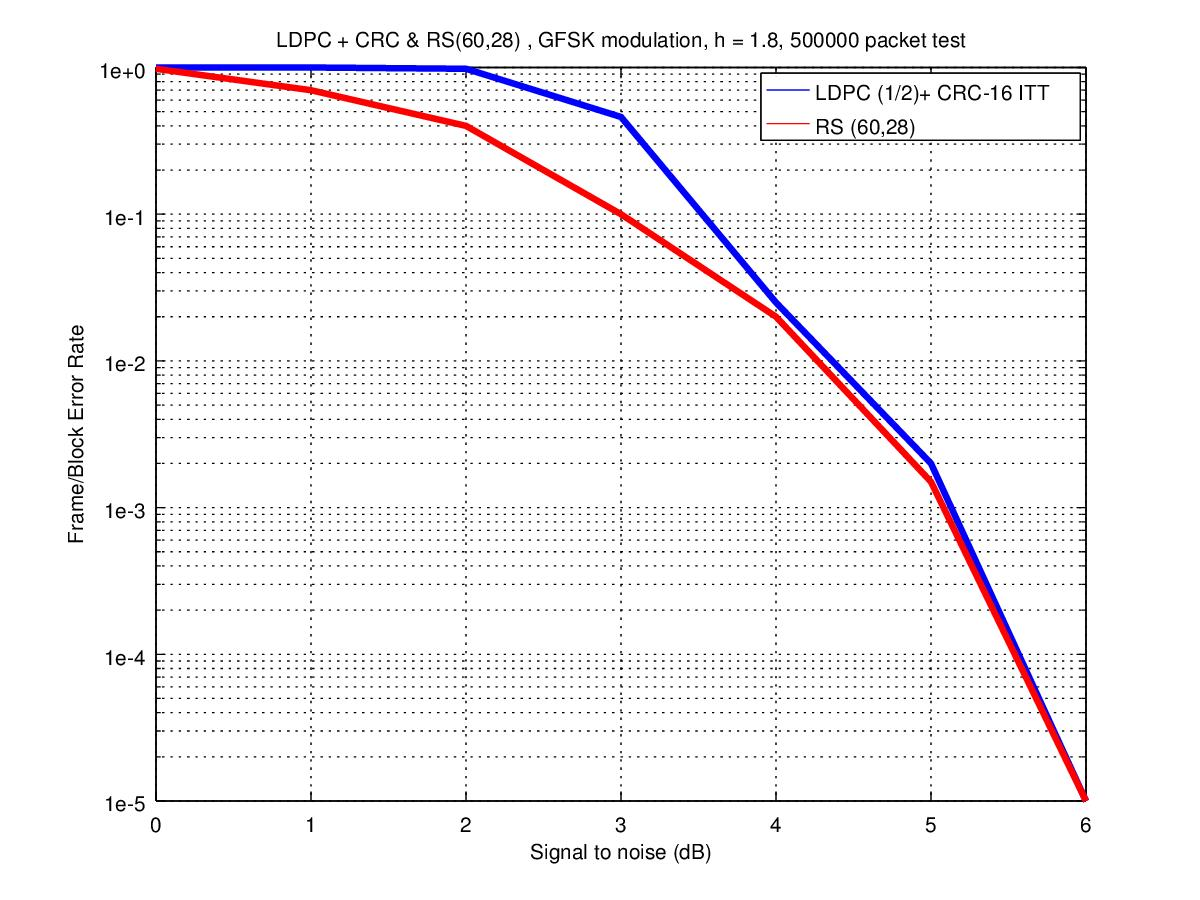
\includegraphics[scale=0.4]{figures/LDPC_RS.jpg}
%
%  \end{frame}
  
  %%%%%%%%%%%%%%%%%%%
  
%%%%%%%%%%%%%%%%%%%


%%%%%%%%%%%%%%%

%%%%%%%%%%%%%%%%%%%

\section{Conclusion}

\begin{frame}{Conclusion}
\begin{itemize}
 
\item Les Travaux de recherche dovient avoir toujours à la tête les aspects et contraintes pratiques.  
\item La Simulation est un trés bons moyen pour avoir un preuve théorique Mathèmatique.
\item Les Nouvelle Propositions des canaux et Nouveaux Codage du canal peut utiliser au sein de protocole de DASH7.
\item Les Autres développements peut se faire au future comme avoir un Relay, Egaliseur, Software Defined Radio ... .
\end{itemize}

\end{frame}

%%%%%%%%%%%%%%%%%%%%%%%

\begin{frame}



\begin{figure}[h!]
  \centering
    
\includegraphics[scale=0.5]{figures/merci.jpg}
\end{figure}



\end{frame}




\begin{thebibliography}{9}

\bibitem{errorcontrolcoding} 
Shu Lin, Daniel J.Costello, Jr. 
\textit{Error Control Coding}. (Second Edition), 2004.

\end{thebibliography}


\end{document}